\documentclass{foi}
\usepackage{lipsum}
\usepackage[utf8]{inputenc}
\usepackage{float}

\lstset{basicstyle=\ttfamily,
  showstringspaces=false,
  commentstyle=\color{red},
  keywordstyle=\color{blue},
}

\vrstaRada{\zavrsni}
\title{Izrada aplikacije za pronalazak termina sastanaka}

\author{Leo Ćavar}
\spolStudenta{\musko}
\mentor{Marko Mijač}
\spolMentora{\musko}
\godina{2024}
\mjesec{Rujan}
\date{2024}
\status{redoviti}
\indeks{0016153823}
\smjer{Informacijski i poslovni sustavi}
\titulaProfesora{Doc. Dr. sc.}

\sazetak{U ovom završnom radu se obrađuje korištenje .NET tehnologija za izradu programa za dogovaranje sastanka. Kroz rad se obrađuje kratko o ASP. NET Core i ASP. NET Web API tehnologijama, kao i koncepte API-ja i HTTP metoda, Google API-ja, uključujući Google Calendar API, autentifikaciju i autorizaciju korisnika pomoću OAuth 2.0 protokola, te primjere zahtjeva za dohvaćanje i upravljanje kalendarskim događajima kroz implementaciju .NET web aplikacije 
}

\kljucneRijeci{API; ASP. NET Core; .NET; C\#; ASP. NET; ; OAuth 2.0; Google Calendar; Google API;}

\begin{document}

\maketitle

\tableofcontents

\pagestyle{plain}
\chapter{Uvod}
U ovom radu ćemo se usredotočiti na izradu programa za dogovaranje sastanaka kroz upotrebu Google API-ja, koji nam omogućava interakciju s iznimno popularnim Google kalendarom. Realizirat ćemo program koristeći ASP.NET Core i Razor stranice za izradu front-end sučelja te upravljanje podacima, dok će ASP.NET Web API služiti za primanje HTTP zahtjeva i komuniciranje s Google servisima za manipuliranje događajima.

\chapter{Metode i tehnike rada}
Za pisanje teksta i formatiranje ovog rada koristio se LaTeX unutar programa Visual Studio Code. Za izradu praktičnog dijela korišten je Visual Studio 2022 i JetBrains Rider.

\chapter{API}
Kada korisnik koristi softver kao klijent, često koristi nekakvo softversko sučelje za interakciju s softverom, ali kada je potrebno da jedan softver koristi dijelove drugog softvera tada koristimo vrstu sučelja za programiranje aplikacija (engl. \textit{Application Programming Interface}) ili skraćeno API.\cite{biehl2015api}
Ta interakcija se najčešće bazira na tome da klijent šalje HTTP zahtjev serveru na određenu lokaciju i dobivaju se nazad podaci.
API zahtjev se sastoji od nekoliko dijelova \cite{altexsoft}
\begin{itemize}
    \item Operacija koja se izvršava (primjer. \textit{GET, POST})
    \item Autentifikacijski parametri
    \item Odredište - URL API završne točke (engl. \textit{endpoint})
\end{itemize}
Poziv može sadržavati i druge parametre ali ovo su tri osnovna koja će se uvijek koristiti.
\section{HTTP zahtjevi}
Kada klijent šalje zahtjev poslužitelju mora specifirati u zahtjevu koju metodu želi izvršiti, imena metoda se odnose na ono što želimo postići sa zahtjevom. \cite{Maurya2021} 
\begin{itemize}
    \item \textbf{GET} metoda se koristi za dohvaćanje podataka
    \item \textbf{POST} - slanje i dodavanje podataka
    \item \textbf{PUT} - Ažuriranje podataka
    \item \textbf{DELETE} - brisanje resursa 
\end{itemize}

\section{RESTFul API}
RESTFul API je vrsta API-ja koja prati REST \textit(eng. {representational state transfer}) principe dizajna, može biti u bilo kojem jeziku i može koristiti bilo koju vrstu podataka \cite{ibm_rest_api}.
Iako najčešće koristi HTTP protokol on nije nužno vezan za njega.\cite{Microsoft2023}
\begin{itemize}
    \item \textbf{Jedinstveno sučelje} - API dizajn mora biti konzistentan i predvidljiv, s pristupom resursima putem standardnih HTTP metoda kao što su GET, POST, PUT i DELETE.
    
    \item \textbf{Razdvajanje klijenta i servera} - Klijent i server su neovisni, gdje server ne čuva informacije o stanju klijenta između zahtjeva, a klijent nema direktan pristup serverovim podatcima.
    
    \item \textbf{Bezustanje (engl. \textit{Stateless})} - Svaki zahtjev od klijenta prema serveru mora sadržavati sve potrebne informacije za obradu, bez potrebe za čuvanjem stanja na serveru.
    
    \item \textbf{Keširanje} - Resursi se mogu keširati kako bi se smanjilo opterećenje servera i omogućilo ponovnu upotrebu već preuzetih podataka.
    
    \item \textbf{Sustav slojeva} - Slojevita arhitektura omogućuje umetanje posrednika između klijenta i servera, dodajući funkcionalnosti poput keširanja ili sigurnosnih provjera.
    
    \item \textbf{Kôd na zahtjev (opcionalno)} - Klijent može preuzeti i izvršiti kod od servera radi proširenja funkcionalnosti aplikacije. 
\end{itemize}

\chapter{ASP.NET Core}
\section{ASP.NET MVC}
ASP.NET MVC je framework koji se bazira na MVC (engl. \textit{Model-View-Controller}) arhitekturi, izgrađen je na .NET platformi i koristi se za izradu web aplikacija \cite{Tyler2024}.
Kao što ime glasi, MVC arhitektura se sastoji od modela, pregleda (eng. \textit{View}) i kontrolera (eng. \textit{Controller}). Ovaj oblik dizajna prati prvi princip SOLID metoda, razdvajanja odgovornosti (eng. \textit{Seperation of concerns}).
MVC omogućava ponovnu upotrebljivost, i zbog podjele na 3 glavne komponente olakšava održavanje koda. \cite{GeeksforGeeks2024}
\begin{figure}[H]
    \centering
    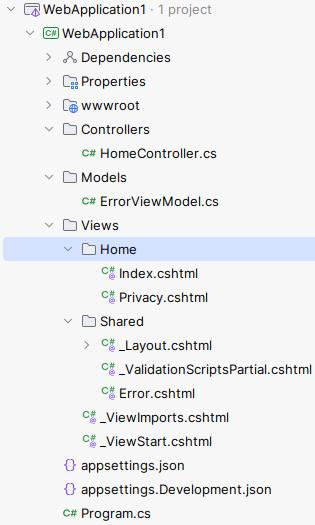
\includegraphics[width=0.6\textwidth]{slike/MVC_project.jpeg}
    \caption{Prikaz MVC u ASP.NET MVC projektu (Izvor: autor)}
    \label{fig:mvc_projekt}
\end{figure}

\subsection{Model}
Unutar konteksta ASP.NET MVC projekta, model predstavlja C\# klasu koja sadrži svojstva za spremanje podataka kojima upravljamo. Model je neovisan o korisničkom sučelju ali često će postojati pregled (engl. textit{View}) koji odgovara za prikaz i upravljanje modelom.
Model također može sadržavati poslovnu logiku za upravljanje podacima, iako to nije učestala praksa i često se ta uloga daje servisima.
\subsection{View}
Pregledi (eng. \textit{Views}) se koriste za prikazivanje podataka i korisničku interakciju. ASP.NET MVC koristi Razor stranice, sa ekstenzijom \textit{cshtml}. Razor stranice omogućavaju pisanje C\# koda unutar HTML datoteka koji služi za interaktiranje sa HTML oznakama za generiranje web sadržaja \cite{Smith2022}. Najčešće će svaki pregled imati svoj kontroler koji je odgovoran za rad s pregledima.

\subsection{Controllers}
Kontroler u ASP.NET Core MVC arhitekturi služi kao posrednik između modela i prikaza. On obrađuje korisničke zahtjeve, upravlja podacima iz modela, i odlučuje koji će prikaz biti vraćen korisniku. Kontroleri su ključni dio MVC uzorka jer povezuju poslovnu logiku s korisničkim sučeljem.
Kontroler je klasa koja obično nasljeđuje baznu klasu \texttt{Controller} i sadrži metode koje se nazivaju akcije (engl. \textit{actions}). Svaka akcija odgovara određenom korisničkom zahtjevu i vraća rezultat, kao što je prikaz (\textit{ViewResult}), JSON podaci (\textit{JsonResult}), ili redirekcija (\textit{RedirectResult}).
Akcije također možemo opisati kao metode koje se povezivaju kad unesemo određeni URL. \cite{Walther2022}

\section{ASP.NET Web API}
ASP.NET Core nam omogućava da kreiramo web API s upotrebom kontrolera koji su usredočeni na resurse i primanje HTTP zahtjeva. Prednost kreiranja zasebnog Web API projekta je da ga može koristiti više različitih vrsta klijenta.\cite{ASPNet2023}
U ASP.NET Core možemo imati dva pristupa kreiranja API-ja:
\begin{itemize}
    \item \textbf{API bazirani na kontrolerima (engl. \textit{controller-based APIs})}: U ovom pristupu, kontroleri (engl. \textit{controllers}) su klase koje nasljeđuju \texttt{ControllerBase} klasu. Ove klase koriste se za definiranje API krajnjih točaka (engl. \textit{endpoints}). Metode unutar kontrolera mapiraju se na određene HTTP zahtjeve (engl. \textit{HTTP requests}, npr. GET, POST) i vraćaju odgovore u obliku JSON-a, XML-a, ili drugih formata.

    \item \textbf{Minimalni API-ji (engl. \textit{minimal APIs})}: Ovaj pristup omogućava definiranje krajnjih točaka pomoću lambda izraza (engl. \textit{lambda expressions}) ili metoda, bez potrebe za punom klasom kontrolera. Minimalni API-ji su dizajnirani za jednostavne i brze implementacije, gdje se fokusira na definiranje krajnjih točaka uz minimalno opterećenje infrastrukture.
\end{itemize}
Za potrebe ovog rada koristit će se API bazirani na kontrolerima zbog bolje organizacije koda u cjeline te zbog jednostavnijeg rukovanja ulaznim podacima pomoću atributa \textit{[FromBody]} i \textit{[FromQuery]} 

\chapter{Praktični rad: Meeting Planner}
\section{Uvod u projekt}
Prije izrade projekta trebaju se definirati funckionalnosti projekta. Cilj aplikacije je dohvaćanje svih dostupnih termina koje korisnik ima u svome Google kalendaru te sinkronizacija u jedan ispis koji će organizatoru sastanka prikazati kada su dostupni svi planirani korisnici i odabrana dvorana u kojoj će se sastanak održati. 
Na bazi toga, definiramo funckionalnosti.
\begin{itemize}
    \item Prijava korisnika: Korisnik se može prijaviti u sustav koristeći svoje Google podatke.
    \item Prikaz kalendara jednog korisnika (organizator): Korisniku se prikazuje njegov osobni kalendar s pregledom svih zakazanih sastanaka u obliku tablice.
    \item Upis termina u kalendare (kalendar organizatora i kalendar korisnika): Nakon pronalaska slobodnog termina, sustav će omogućiti organizatoru upis sastanka u svoj kalendar kao i njihove kalendare.
    \item Pronalazak slobodnih termina: Sustav pretražuje slobodne termine za sastanak uzimajući u obzir slobodno vrijeme sudionika, odabrane dane za sastanak i dostupne lokacije.
\end{itemize}
Za omogućavanje integracije s Google kalendarom koristiti ćemo Google Calendar API. RESTFul API s kojim se može interaktirati pomoću HTTP poziva.
\section{Google Workspace}
Google Workspace nam omogućava platformu za integraciju Google Workspace alata kao što su Maps, Calendar ili Sheets. Za ovaj projekt su nam potrebni Google Workspace APIs da integriramo kalendar s našim rješenjem.
Da možemo koristiti te servise moramo prvo stvoriti projekt u Google Cloud konzoli te omogućiti Google Calendar API za naš projekt.
\begin{figure}[H]
    \centering
    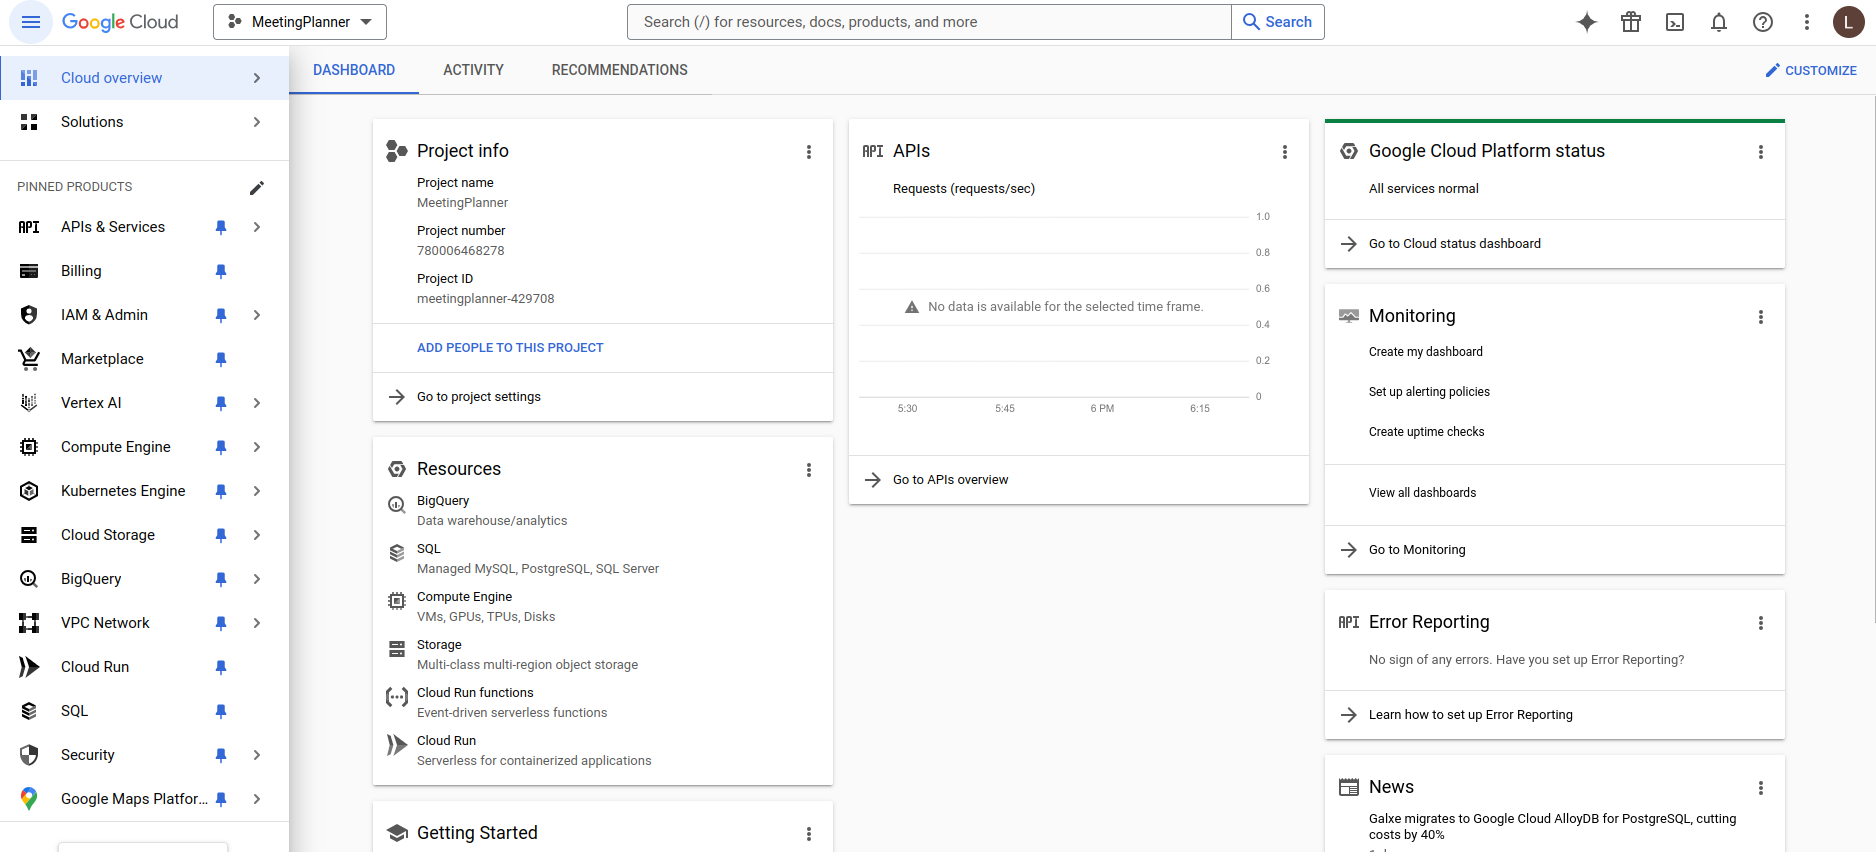
\includegraphics[width=0.9\textwidth]{slike/google_console.png}
    \caption{Google Cloud console (Izvor: autor)}
    \label{fig:google_console}
\end{figure}
\section{Stvaranje projekta}
Za stvaranje projekta prvo je potrebno stvoriti prazno rješenje (engl. \textit{Solution}), te kreirati zasebni WEB API i MVC projekt.
\begin{figure}[H]
    \centering
    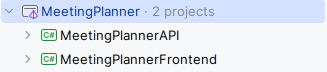
\includegraphics[width=0.6\textwidth]{slike/struktura.png}
    \caption{Rješenje MeetingPlanner (Izvor: autor)}
    \label{fig:struktura}

\end{figure}
Za dodatnu konfiguraciju potrebno je preuzeti json datoteku koja sadrži podatke koji našoj aplikaciji omogućuju pozivanje google servisa. 
\begin{itemize}
    \item GoogleId (Identifikator klijenta): jedinstveni identifikator dodijeljen aplikaciji od strane Googlea. Identificira vašu aplikaciju na Googleovim poslužiteljima prilikom slanja zahtjeva, kao što su autentifikacija korisnika ili pristup API-jima.
    \item GoogleSecret (Tajni ključ): povjerljivi ključ povezan s vašom Google aplikacijom. Koristi se zajedno s GoogleId za autentifikaciju vaše aplikacije prema Googleu.
\end{itemize}
\newpage
\section{Autentifikacija}
Kako bi korisnik aplikacije mogao pristupiti vanjskim uslugama on mora biti prijavljen, korisnik će se prijavljivati putem svojeg Google računa koristeći OAuth 2.0 protokol. Prvo je potrebno konfigurati autentifikaciju projekta u \textit{Program.cs} datoteci.
\begin{figure}[H]
    \centering
    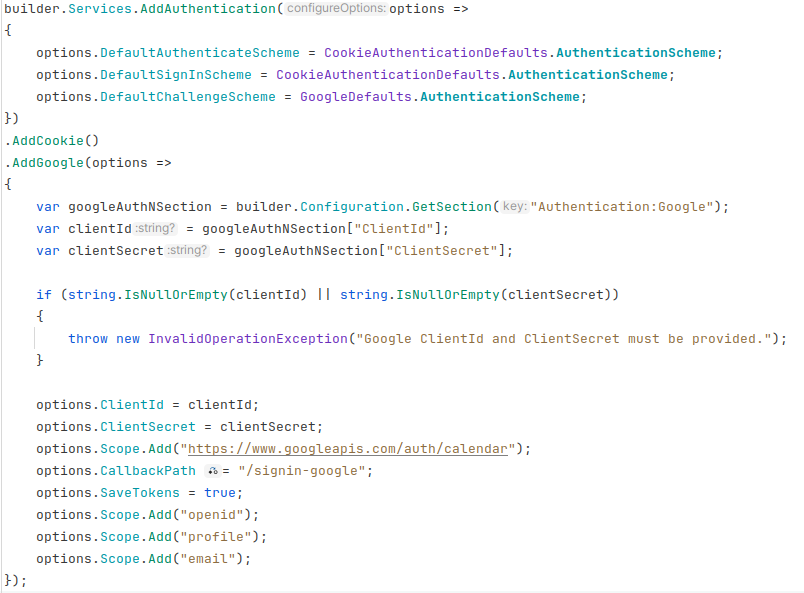
\includegraphics[width=0.7\textwidth]{slike/auth.png}
    \caption{Postavljanje autentifikacije (Izvor: autor)}
    \label{fig:autentifikacija_programcs}
\end{figure} Kod konfigurira autentifikaciju postavljanjem kolačića za prijavu i koristeći Google za autentifikaciju korisnika, uključujući konfiguraciju za Google kalendar, pohranu OAuth tokena, i određivanje putanje za povratak korisnika nakon prijave.
Kada je postavljena konfiguracija kreiramo login stranicu, s obzirom da koristimo Google autentifikaciju kreiramo element koji poziva akciju \textit{LoginWithGoogle}.
\begin{figure}[H]
    \centering
    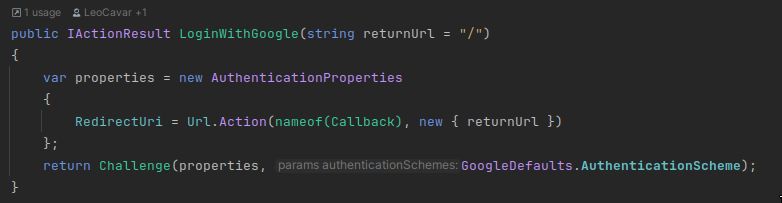
\includegraphics[width=0.9\textwidth]{slike/loginwithgoogle.png}
    \caption{Metoda LoginWithGoogle (Izvor: autor)}
    \label{fig:LoginWithGoogle}

\end{figure}
\newpage
Metoda \textit{LoginWithGoogle} inicijalizira objekt \textit{AuthenticationProperties} s postavkom \textit{RedirectUri} koja određuje putanju na metodu \textit{Callback} nakon prijave putem Googlea. Metoda \texttt{Challenge} pokreće izazov za autentifikaciju koristeći Google kao pružatelja, preusmjeravajući korisnika na Google za prijavu ako nije već prijavljen. Nakon uspješne prijave, korisnik će biti vraćen na metodu \texttt{Callback} gdje se token sprema u sesiju što nam omogućava autorizirane API pozive.
\begin{figure}[H]
    \centering
    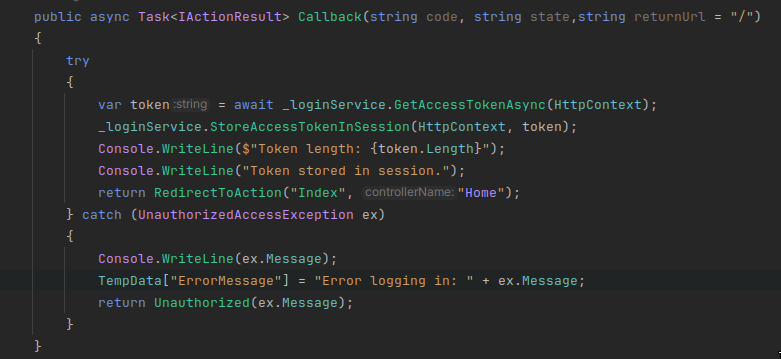
\includegraphics[width=0.9\textwidth]{slike/callbackFunction.png}
    \caption{Metoda Callback (Izvor: autor)}
    \label{fig:Callback}

\end{figure}
Za spremanje podataka u sesiju definira se metoda \textit{StoreAccessTokenInSession}. Metoda se nalazi u zasebnom login servisu unutar kojega se također nalazi metoda za dohvaćanje tokena za kasniju upotrebu \textit{GetAccessTokenAsync}.
\begin{figure}[H]
    \centering
    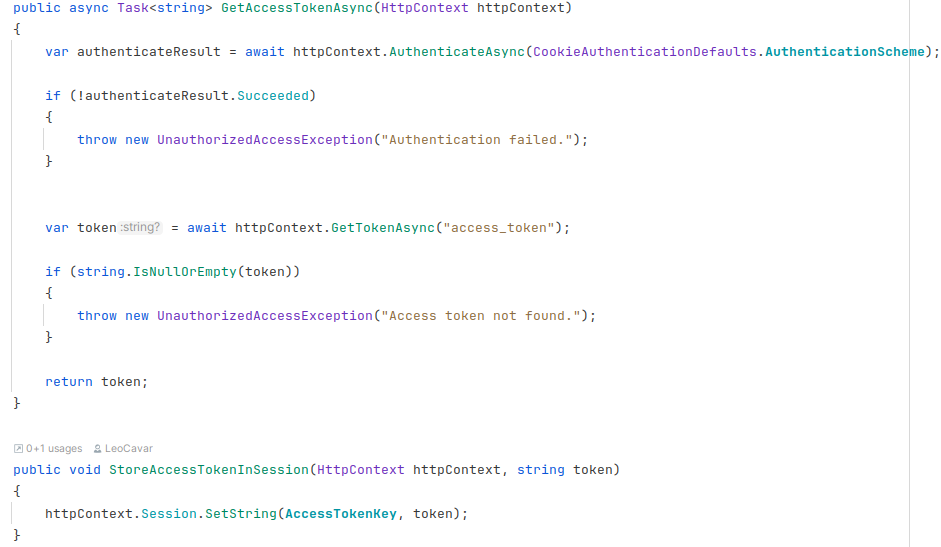
\includegraphics[width=0.9\textwidth]{slike/storeToken.png}
    \caption{Login servis (Izvor: autor)}
    \label{fig:StoreAccessTokenInSession}

\end{figure}






\section{Prikaz događaja}
Za prikaz događaja implementiramo zaseban pregled {eng.\textit{View}}. Koristiti će se mogućnost razor stranica da se upisuje C\# kod i definirat će se jednostavna provjera varijable \textit{isLoggedIn}. 
\begin{figure}[H]
    \centering
    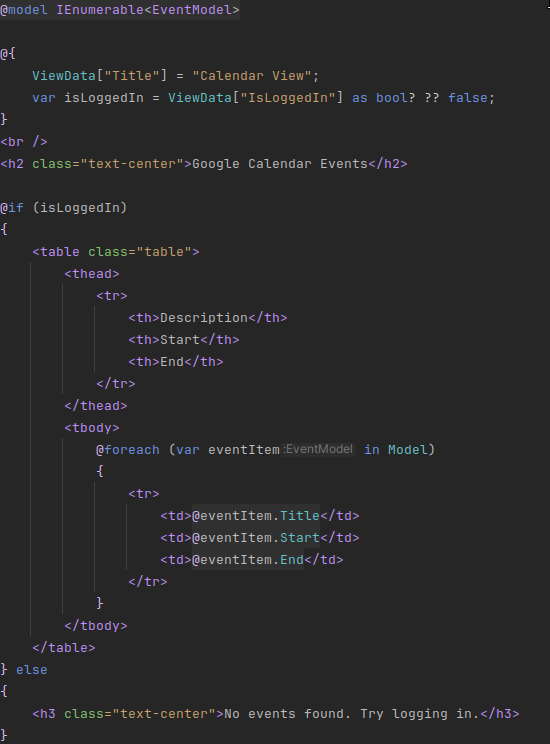
\includegraphics[width=0.6\textwidth]{slike/calendarView.png}
    \caption{Pregled kalendara (Izvor: autor)}
    \label{fig:calendarView}

\end{figure}
Definira se klasa \textit{EventModel} koja sadrži naslov, vrijeme početka i vrijeme kraja događaja. Klasa služi za mapiranje događaja koje dobivamo pozivom API-ju u korisniku lako čitljiv oblik. 
Nakon definiranja ispisa događaja, potrebno je implementirati logiku unutar kontrolera i servisa. Kontroler nam služi za obradu zahtjeva dok se sva poslovna logika i interakcija s podacima izvršava u servisu {\textit{CalendarService}}.
\begin{figure}[H]
    \centering
    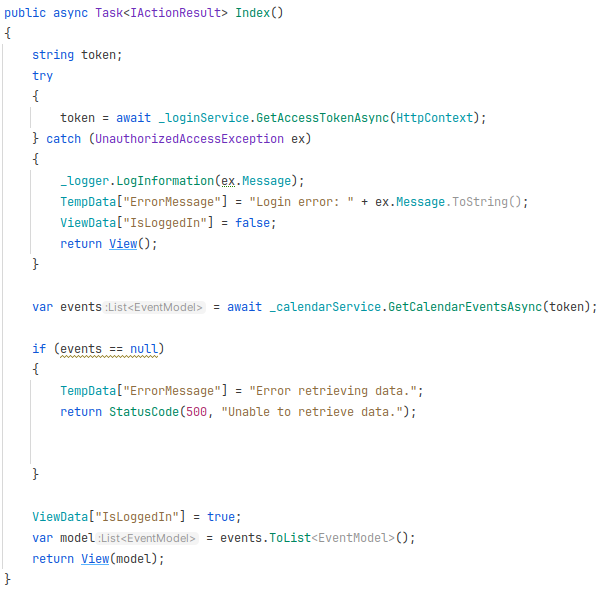
\includegraphics[width=0.9\textwidth]{slike/cControllerIndex.png}
    \caption{Pregled kalendara kontroler (Izvor: autor)}
    \label{fig:ctrl}

\end{figure}
Kontroler dohvaća token pomoću funkcije \textit{GetAccessTokenAsync} te poziva metodu \textit{GetCalendarEventsAsync} koristeći token da pošalje poziv API-ju te upravlja greškama koristeći try/catch metode. 
Unutar \textit{CalendarService} metoda \textit{GetCalendarEventsAsync} stvara klijent pod imenom "API", to je klijent koji sadrži putanju na backend koji sadrži API endpointove.
Zahtjevu se dodaje token u \textit{AuthenticationHeaderValue} da se mogu dohvatiti podaci i šalje se zahtjev na definirani endpoint "\textit{calendar/events}"
\begin{figure}[H]
    \centering
    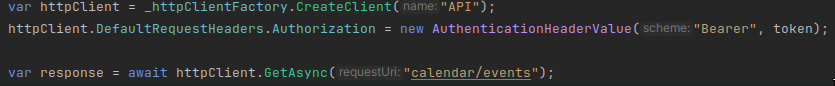
\includegraphics[width=0.9\textwidth]{slike/calendarRequest.png}
    \caption{Slanje zahtjeva na API endpoint za dohvaćanje kalendara (Izvor: autor)}
    \label{fig:calendarRequest}

\end{figure}
Odgovor se mapira iz JSON stringa u .NET objekt, u ovom kontekstu se pretvara u \textit{EventModel}.
\begin{figure}[H]
    \centering
    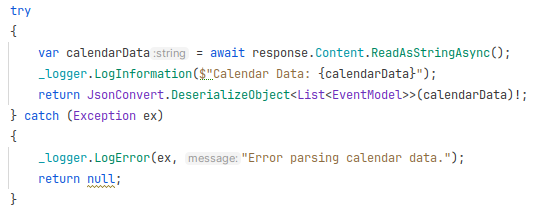
\includegraphics[width=0.9\textwidth]{slike/calendarReturn.png}
    \caption{Metoda za upravljanjem povratnog JSON teksta (Izvor: autor)}
    \label{fig:calendarReturnList}

\end{figure}
Ovo je sva potrebna logika za prednji dio sustava {engl. \textit{Frontend}}. Potrebno je implementirati pozadinski dio {eng. \textit{Backend}}.
Pozadinski dio se implementira tako što se definira \textit{ApiController} ruta koja se pozvala u metodi \textit{GetCalendarEventsAsync}. 
Prvobitno se izvršava validacija tokena te se dohvaćaju događaji pomoću metode \textit{GetSimpleEventsAsync} i provjerava se uspješnost operacije.
\begin{figure}[H]
    \centering
    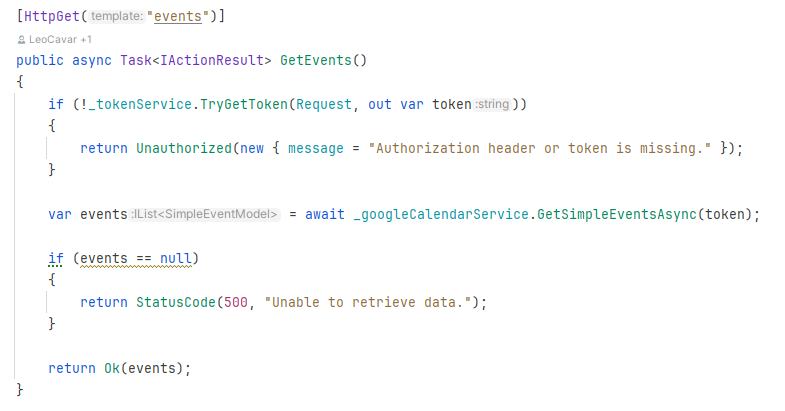
\includegraphics[width=0.9\textwidth]{slike/GetCalendarEventsEndpoint.png}
    \caption{Kalendar "events" endpoint (Izvor: autor)}
    \label{fig:GetCalendarEventsEndpoint}

\end{figure}
Metoda za dohvaćanje se sastoji od dva dijela, prvi dio je stvaranje instance \textit{CalendarService}. Ovaj servis je od GoogleAPI-ja te nam omogućava manipulaciju podacima autoriziranog korisnika unutar google kalendara.
\begin{figure}[H]
    \centering
    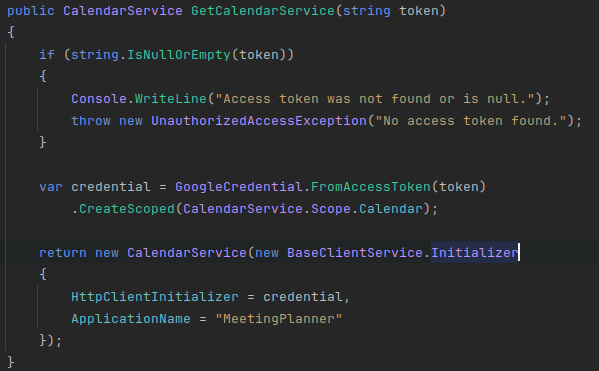
\includegraphics[width=0.9\textwidth]{slike/GetCalendarService.png}
    \caption{Metoda za dohvaćanje instance Google kalendar servisa (Izvor: autor)}
    \label{fig:GetCalendarService}

\end{figure}
Drugi dio procesa je dohvaćanje \textit{Events.List} resursa i mapiranje u obliku \textit{SimpleEventModel}.
\begin{figure}[H]
    \centering
    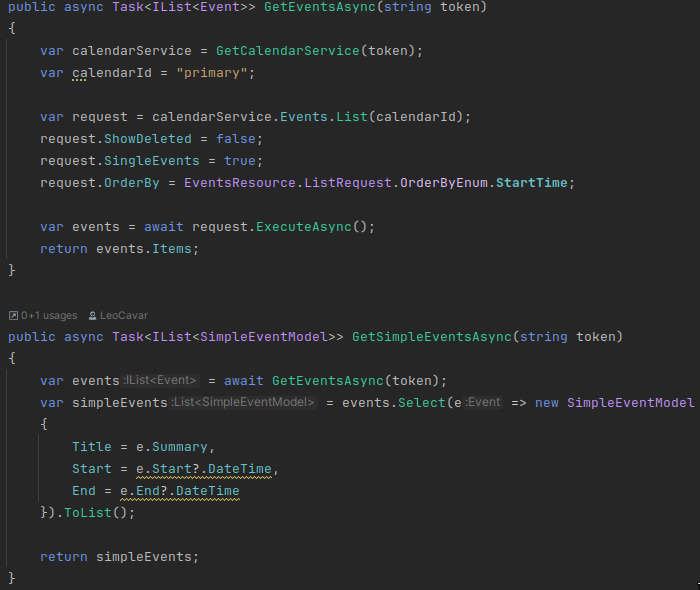
\includegraphics[width=0.8\textwidth]{slike/GetSimpleEventAsync.png}
    \caption{Metoda GetSimpleEventAsync (Izvor: autor)}
    \label{fig:GetSimpleEventAsync}
\end{figure}
Nakon implementacije metode naša funkcionalnost je potpuna, te se kalendar vraća u obliku tablice prijavljenom korisniku.
\begin{figure}[H]
    \centering
    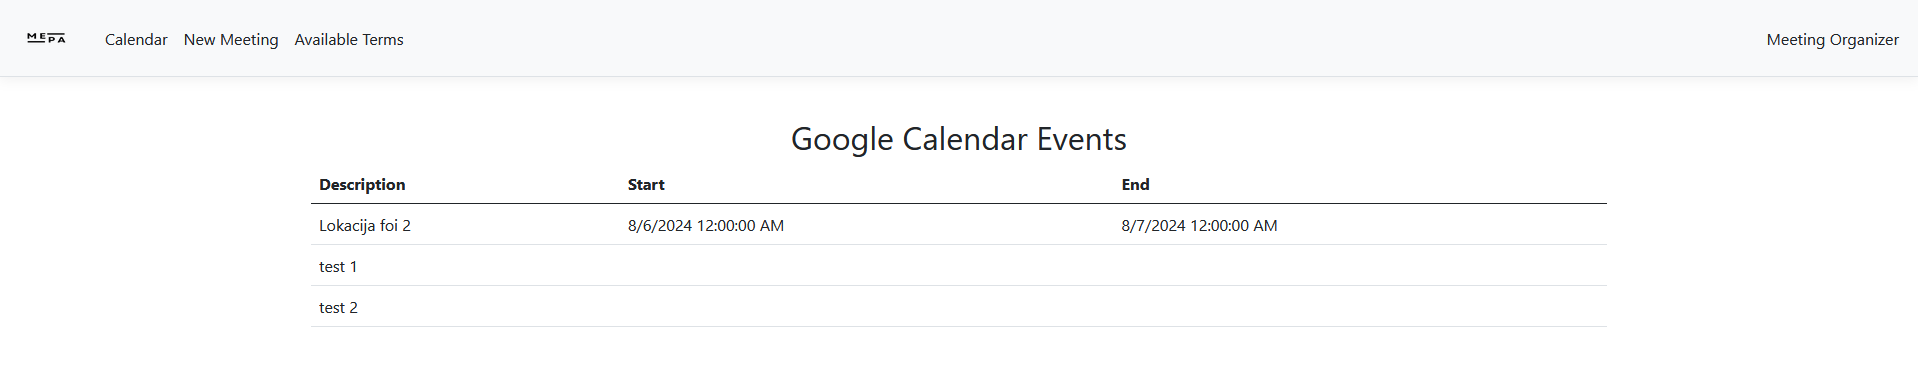
\includegraphics[width=0.8\textwidth]{slike/calendarEvents.png}
    \caption{Prikaz kalendara na web stranici (Izvor: autor)}
    \label{fig:CalendarViewImg}
\end{figure}
\subsection{Protok podataka}

Protok podataka u ovoj aplikaciji je jasno definiran za sve funkcionalnosti koje će se implementirati dalje u ovome radu s malim razlikama ovisno o funkcionalnosti ali uzorak će ostati isti.
\begin{itemize}
    \item \textbf{Klijentov zahtjev}: Korisnik putem web aplikacije odabire funkcionalnost koju želi koristiti putem korisničkoj sučelja te se šalje odgovarajući zahtjev
    \item \textbf{Obrada zahtjeva na poslužitelju}: Poslužiteljski kontroler prima zahtjev i prosljeđuje ga odgovarajućem servisu.
    \item \textbf{Autentifikacija i autorizacija}: Prilikom dohvaćanja podataka iz Google Calendar API-ja, aplikacija koristi OAuth 2.0 autentifikaciju. Token za pristup provjerava se i koristi za autentifikaciju zahtjeva prema Googleovim uslugama.
    \item \textbf{Odgovor poslužitelja}: Nakon obrade podataka, poslužitelj šalje odgovor klijentu. Ovaj odgovor uključuje popis slobodnih termina za sve korisnike u traženom vremenskom periodu, koji se klijentu vraćaju u JSON formatu ili potvrdu o izmjeni i unosu podataka.
    \item \textbf{Prikaz rezultata klijentu}: Klijentska aplikacija prima JSON odgovor i prikazuje slobodne termine korisniku u vizualno preglednom formatu, omogućujući mu da jednostavno vidi kada su svi korisnici dostupni ili se prikazuje odgovarajuća greška ovisno o odgovoru.
\end{itemize}

\section{Pronalazak slobodnih termina}
Kako Google Calendar API ne omogućuje izravno dohvaćanje slobodnih termina, postupak pronalaska slobodnih perioda obuhvaća sljedeće korake:
\begin{itemize}
    \item Dohvat kalendara svih dolaznika (engl. \textit{Attendees})
    \item Filtriranje kalendara po lokaciji
    \item Identificiranje zauzetih termina unutar zadanog vremenskog raspona
    \item Kombiniranje svih zauzetih termina kako bi se pronašli zajednički slobodni periodi
    \item Oduzimanje zauzetih termina od cijelog vremenskog raspona kako bi se identificirali slobodni termini
\end{itemize}

\newpage
Korisničko sučelje uključuje obrazac koji šalje zahtjev na \textit{calendar/get-available-times} nakon unosa podataka. Odgovor se prikazuje u tablici sa slobodnim periodima.

\begin{figure}[H]
    \centering
    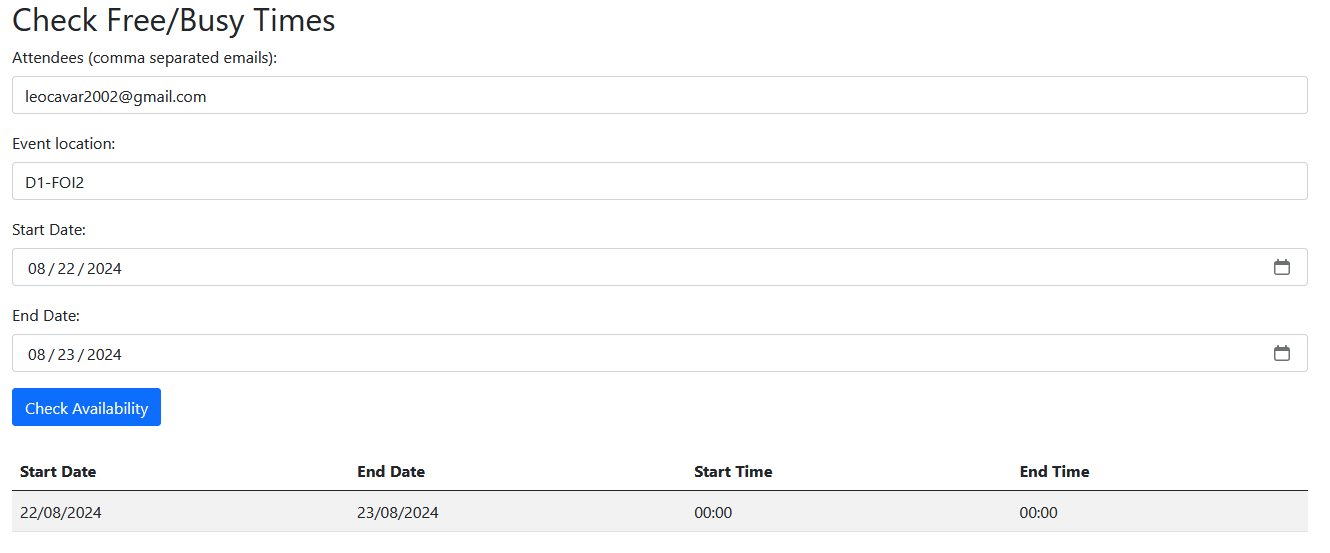
\includegraphics[width=0.7\textwidth]{slike/timesAvaileble.png}
    \caption{Web sučelje za prikaz dostupnih termina (Izvor: autor)}
    \label{fig:UserInterfaceAvailible}
\end{figure}

Funkcija \textit{GetAvailableTimesAsync} vraća popis objekata \textit{TimePeriod} koji sadrži vrijeme početka i kraja slobodnog perioda. Zahtjev uključuje token u headeru, a u tijelu se nalaze vremenski period, lokacija i email adrese korisnika. Funkcija šalje POST zahtjev na \textit{get-available-times} endpoint, koji zatim prosljeđuje zahtjev metodi \textit{GetCommonFreePeriodsWithLocation} nakon validacije tokena i zahtjeva.
Unutar akcije \textit{GetAvailableTimes} na koju se šalje zahtjev dohvaćaju se prvo svi termini kada su korisnici zauzeti.
\begin{figure}[H]
    \centering
    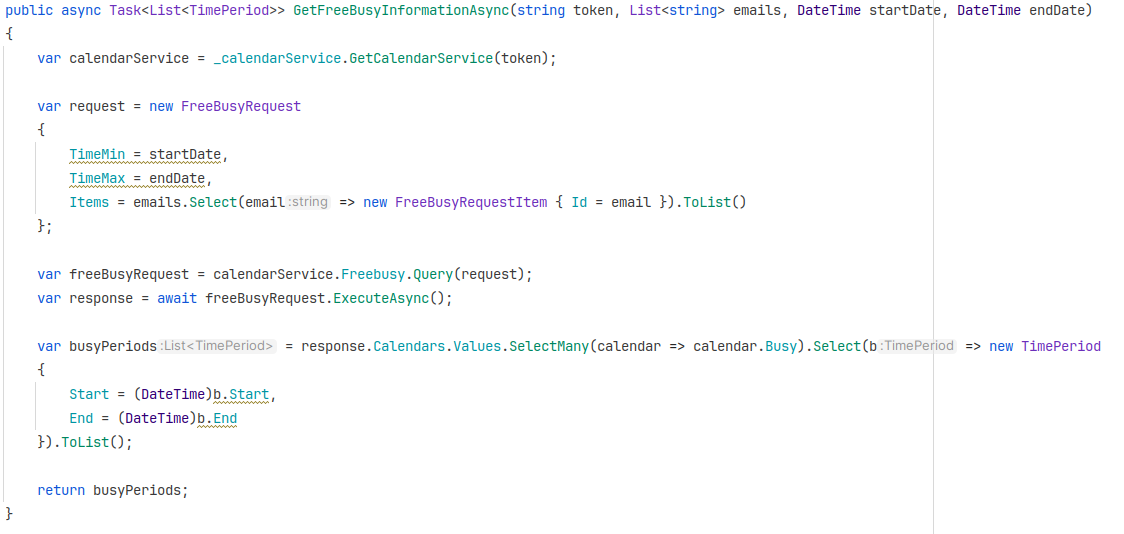
\includegraphics[width=0.7\textwidth]{slike/getfreebuisy.png}
    \caption{Metoda \textit{GetFreeBusyInformationAsync} (Izvor: autor)}
    \label{fig:GetFreeBusyInformationAsync}
\end{figure}
Nakon dohvaćanja zauzetih termina za sve korisnike, potrebno je preuzeti termine kada je dvorana zauzeta.
\begin{figure}[H]
    \centering
    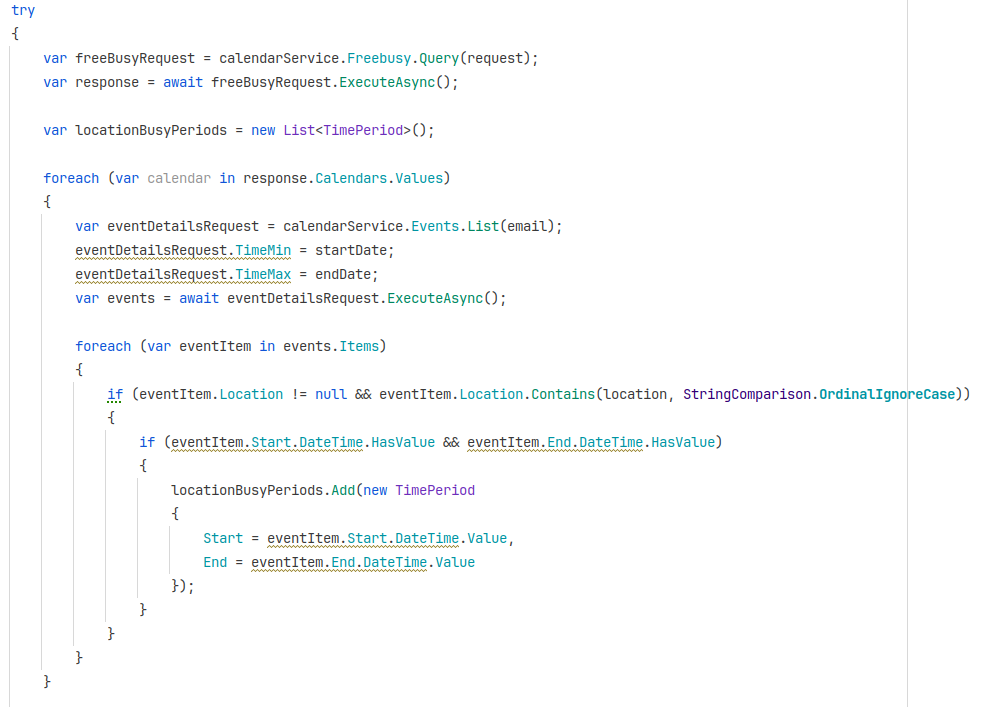
\includegraphics[width=0.7\textwidth]{slike/GetBuisyLocation.png}
    \caption{Dohvaćanje zauzetih termina odabrane lokacije (Izvor: autor)}
    \label{fig:GetBuisyLocation}
\end{figure}
Nakon preuzimanja termina lokacije imamo sve potrebne podatke, prvo je potrebno spojiti zauzete periode korisnika s zauzetim terminima dvorane, metoda \textit{Concat} omogućava da spojimo periode u jednu varijablu \textit{combinedBusyPeriods}.
Nakon spajanja u jednu varijablu, moramo pretvoriti popis zauzetih termina u popis slobodnih termina. Implementira se metoda \textit{GetCommonFreePeriods} i kao povratna vrijednost klijentu se vraćaju svi slobodni periodi.
\begin{figure}[H]
    \centering
    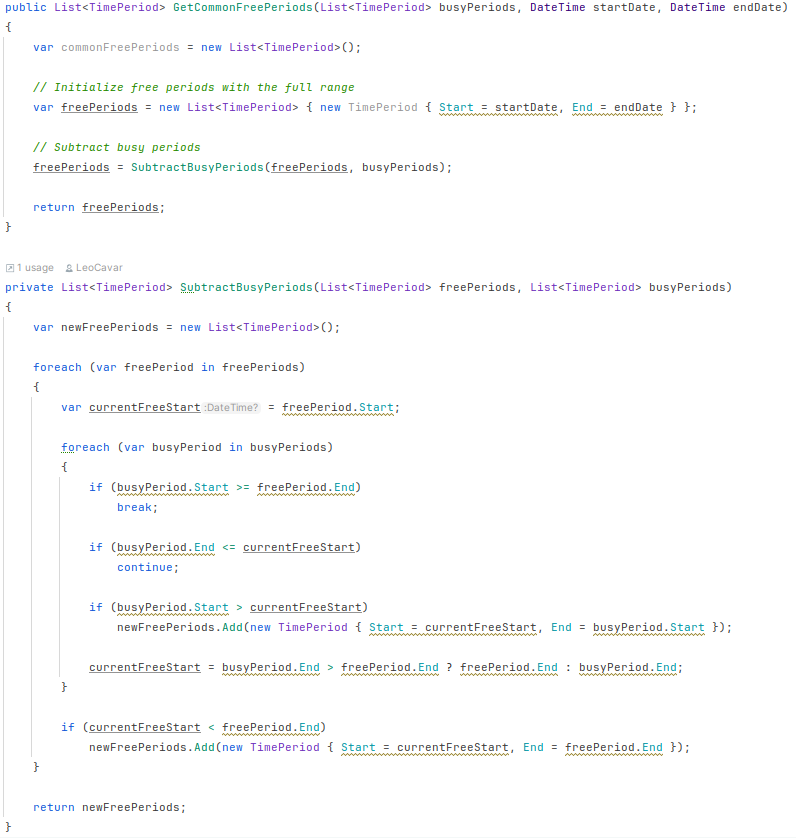
\includegraphics[width=0.6\textwidth]{slike/FreePeriods.png}
    \caption{Metode za pretvaranje zauzetih termina u slobodne (Izvor: autor)}
    \label{fig:FreePeriods}
\end{figure}
Metode \textit{GetCommonFreePeriods} i \textit{SubtractBusyPeriods} instanciraju popis \textit{TimePeriod} unutar odabranog vremenskog raspona te pomoću metode \textit{SubtractBusyPeriods} se od slobodnih vremena oduzimaju zauzeta vremena, stvarajući popis u kojemu se nalaze svi slobodni termini korisnika.
\section{Unos sastanka}
Kao završni dio aplikacije potrebno je omogućiti korisniku da unosi aktivnosti u kalendare korisnika. Prvo je potrebno kreirati sučelje za unos, korisnik može unositi opis, lokaciju sastanka, opis , vremenski period aktivnosti, vremensku zonu i goste sastanka.
\begin{figure}[H]
    \centering
    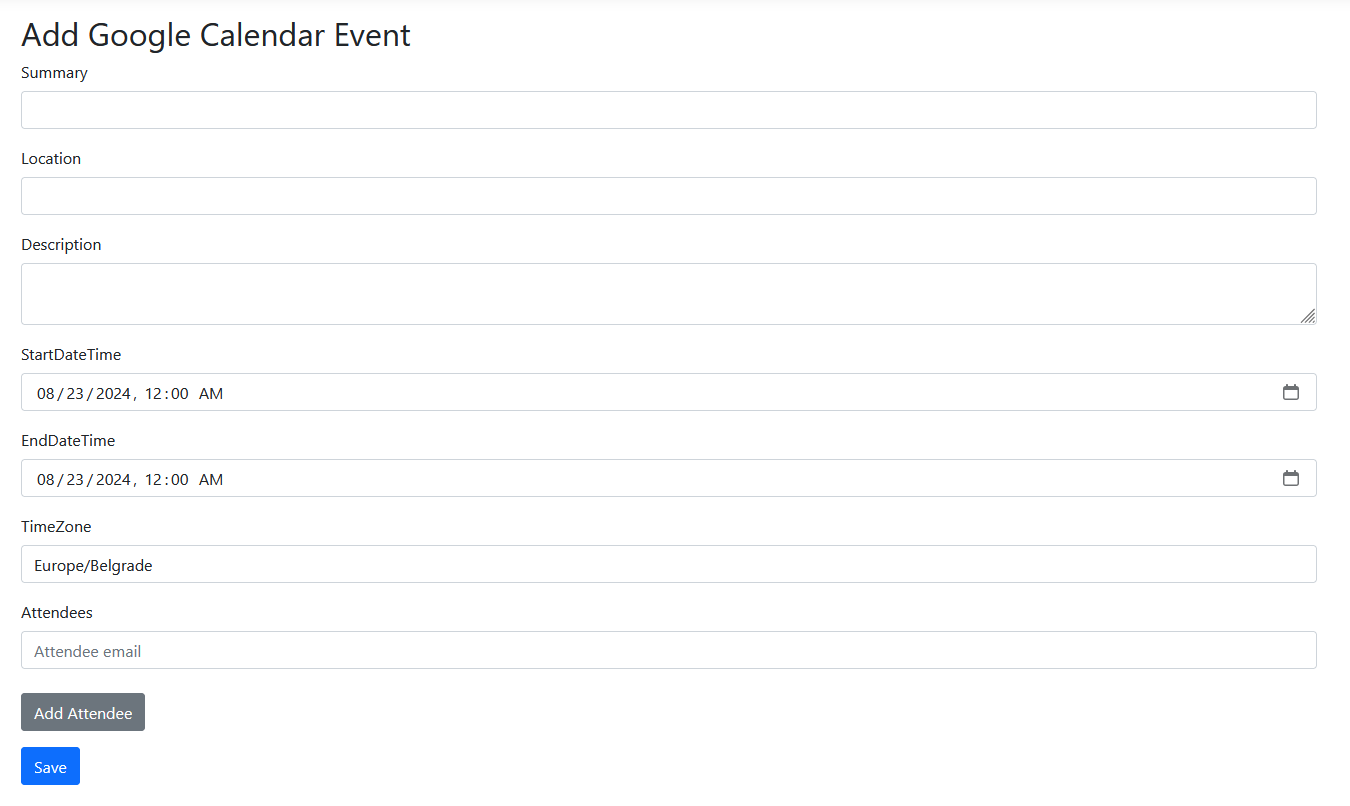
\includegraphics[width=0.8\textwidth]{slike/insertMeeting.png}
    \caption{Sučelje za unos sastanka (Izvor: autor)}
    \label{fig:InsertMeeting}
\end{figure}
Potrebno je poslati POST zahtjev s svim parametrima, uneseni podaci se mapiraju u klasu \textit{InsertEventModel} te se šalju na \textit{calendar/events} endpoint. Stvara se novi \textit{Event} objekt u kalendaru organizatora, te se na taj događaj dodaju članovi.
\begin{figure}[H]
    \centering
    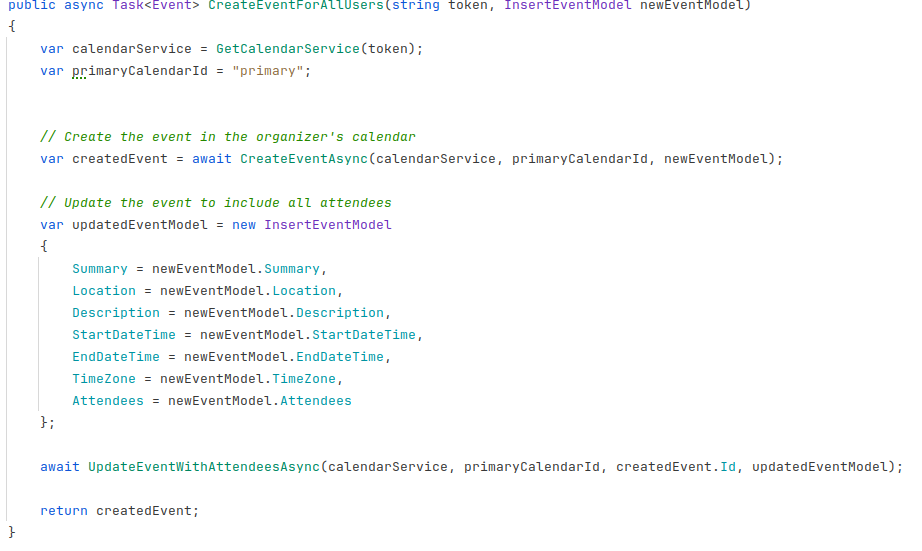
\includegraphics[width=0.8\textwidth]{slike/createEventForAllUsers.png}
    \caption{Implementacija unosa događaja u kalendare korisnika (Izvor: autor)}
    \label{fig:createEventForAllUsers}
\end{figure}




\chapter{Zaključak}
Zaključno, ovaj rad prikazuje proces izrade aplikacije za planiranje sastanaka korištenjem Google Calendar API-ja, razvijene u ASP.NET Core tehnologiji. Kroz detaljno objašnjenje, prikazane su glavne funkcionalnosti aplikacije kao što su autentifikacija korisnika, dohvaćanje događaja iz Google kalendara te prikaz i manipulacija tim događajima. Rad se također osvrće na tehničke aspekte implementacije poput uporabe RESTful API-ja i MVC arhitekture, čime se naglašava važnost modularnosti i razdvajanja odgovornosti u softverskom razvoju. Korištenje Google Workspace API-ja omogućilo je integraciju vanjskih servisa. Aplikacija razvijena u sklopu ovog rada pokazuje kako se napredne tehnike web razvoja mogu iskoristiti za rješavanje konkretnih poslovnih izazova u kontekstu organizacije sastanaka.
\printbibliography[title=Popis literature]
\addcontentsline{toc}{chapter}{Popis literature}

\listoffigures
\addcontentsline{toc}{chapter}{Popis slika}


\end{document}
